% ============================================================
%  Příprava na maturitu – Elektrotechnika
%  Okruh 4: Střídavý proud a kompenzace jalového výkonu
% ============================================================

\documentclass[a4paper,10pt]{article}

\usepackage[T1]{fontenc}
\usepackage[utf8]{inputenc}
\usepackage[left=2.0cm, right=1.8cm, top=1.8cm, bottom=1.8cm]{geometry}
\usepackage{parskip}
\usepackage{xcolor}
\usepackage{tabularx}
\usepackage{booktabs}
\usepackage{tikz}
\usepackage{mdframed}
\usepackage{amsmath}
\usepackage{enumitem}
\usepackage{circuitikz}

\usetikzlibrary{arrows.meta, positioning, decorations.pathmorphing, shapes.geometric, patterns}

% --- Barvy ---
\definecolor{accent}{HTML}{1A3A5C}
\definecolor{lightblue}{HTML}{EAF2F8}
\definecolor{lightyellow}{HTML}{FDFBE4}
\definecolor{lightgreen}{HTML}{EAF7EA}
\definecolor{lightred}{HTML}{FDE8E8}
\definecolor{lightgray}{HTML}{F4F4F4}

% --- Boxy ---
\newmdenv[backgroundcolor=lightblue,linecolor=accent!40,roundcorner=4pt,
  innertopmargin=6pt,innerbottommargin=6pt,innerleftmargin=8pt,innerrightmargin=8pt]{pojmybox}
\newmdenv[backgroundcolor=lightyellow,linecolor=accent!30,roundcorner=4pt,
  innertopmargin=6pt,innerbottommargin=6pt,innerleftmargin=8pt,innerrightmargin=8pt]{vysvetlenibox}
\newmdenv[backgroundcolor=lightgreen,linecolor=accent!40,roundcorner=4pt,
  innertopmargin=6pt,innerbottommargin=6pt,innerleftmargin=8pt,innerrightmargin=8pt]{vzorcebox}
\newmdenv[backgroundcolor=lightred,linecolor=accent!30,roundcorner=4pt,
  innertopmargin=6pt,innerbottommargin=6pt,innerleftmargin=8pt,innerrightmargin=8pt]{durazbox}

\setlist[itemize]{noitemsep, leftmargin=1.4em, topsep=2pt}
\setlist[enumerate]{noitemsep, leftmargin=1.4em, topsep=2pt}

% --- Zkratka pro jednotky ---
\newcommand{\jednotka}[1]{\,[\mathrm{#1}]}

\begin{document}

% ============================================================
\section*{\large Okruh 4 – Střídavý proud a kompenzace jalového výkonu}

\begin{pojmybox}
\textbf{Klíčové pojmy:}
perioda, frekvence, okamžitá a efektivní hodnota, fázový posun, fázor, impedance, reaktance (kapacitní a induktivní), činný, jalový a zdánlivý výkon, účiník, kompenzace účiníku
\end{pojmybox}

\begin{vysvetlenibox}

% ================================================================
\subsection*{1. Základní pojmy střídavého proudu (AC)}

Střídavý proud mění v čase svou velikost i směr. Nejčastějším průběhem je \textbf{sinusoida}.

\begin{vzorcebox}
\[
u(t) = U_m \cdot \sin(\omega t + \varphi) \jednotka{V}
\qquad
\omega = 2\pi f = \frac{2\pi}{T} \jednotka{rad/s}
\]
kde $U_m$ = amplituda, $\omega$ = úhlová frekvence, $T$ = perioda [s], $f$ = frekvence [Hz].
\end{vzorcebox}

\textbf{Efektivní hodnota ($U, I$):} Hodnota střídavého proudu, který by v odporové zátěži vykonal stejnou práci jako proud stejnosměrný. V síti 230\,V je amplituda $U_m \approx 325$\,V.
\begin{vzorcebox}
\[
U = \frac{U_m}{\sqrt{2}} \approx 0{,}707 \cdot U_m
\qquad
I = \frac{I_m}{\sqrt{2}}
\]
\end{vzorcebox}

\begin{center}
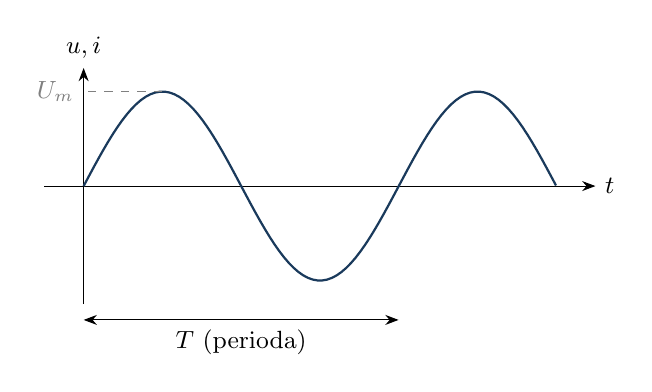
\begin{tikzpicture}[>=Stealth, font=\small]
  % Osy
  \draw[->] (-0.5,0) -- (6.5,0) node[right] {$t$};
  \draw[->] (0,-1.5) -- (0,1.5) node[above] {$u, i$};
  % Sinusoida
  \draw[thick, accent, domain=0:6, samples=100] plot (\x, {1.2*sin(\x*1.57*180/pi)});
  % Popis amplitudy
  \draw[dashed, gray] (1,1.2) -- (0,1.2) node[left] {$U_m$};
  % Perioda
  \draw[<->] (0,-1.7) -- (4,-1.7) node[midway, below] {$T$ (perioda)};
\end{tikzpicture}
\end{center}

% ================================================================
\subsection*{2. Ohmův zákon v obvodech střídavého proudu}

V AC obvodech kladou součástky odpor, který nazýváme \textbf{impedance $Z$}. Ta se skládá z reálné části (\textbf{rezistance $R$}) a imaginární části (\textbf{reaktance $X$}).

\begin{vzorcebox}
\[
U = Z \cdot I \quad \text{(Ohmův zákon pro AC)}
\qquad
Z = \sqrt{R^2 + X^2} \jednotka{\Omega}
\]
\end{vzorcebox}

\textbf{Typy reaktancí:}
\begin{itemize}
  \item \textbf{Induktivní reaktance (cívka):} $X_L = \omega L = 2\pi f L$. Proud se \textbf{zpožďuje} za napětím o $90^\circ$.
  \item \textbf{Kapacitní reaktance (kondenzátor):} $X_C = \frac{1}{\omega C} = \frac{1}{2\pi f C}$. Proud \textbf{předbíhá} napětí o $90^\circ$.
\end{itemize}

% ================================================================
\subsection*{3. Výkony v obvodech střídavého proudu}

Ve střídavých obvodech s reaktivními prvky (L, C) rozlišujeme tři druhy výkonu:

\begin{enumerate}
  \item \textbf{Činný výkon ($P$):} Skutečně vykonaná práce (mění se v teplo nebo mechanickou energii).
  \item \textbf{Jalový výkon ($Q$):} Energie, která se pouze "přelévá" mezi zdrojem a polem (induktivním nebo kapacitním). Nevykonává práci, ale zatěžuje vodiče.
  \item \textbf{Zdánlivý výkon ($S$):} Celkový výkon dodávaný zdrojem.
\end{enumerate}

\begin{vzorcebox}
\[
P = U \cdot I \cdot \cos \varphi \jednotka{W} \text{ (watt)}
\]
\[
Q = U \cdot I \cdot \sin \varphi \jednotka{VAr} \text{ (voltampér reaktanční)}
\]
\[
S = U \cdot I = \sqrt{P^2 + Q^2} \jednotka{VA} \text{ (voltampér)}
\]
\end{vzorcebox}

$\cos \varphi$ se nazývá \textbf{účiník}. Udává, jak velká část zdánlivého výkonu se přemění na činný.

% ================================================================
\subsection*{4. Trojúhelník výkonů a fázorový diagram}

Vztah mezi výkony lze graficky znázornit pomocí pravoúhlého trojúhelníka.

\begin{center}
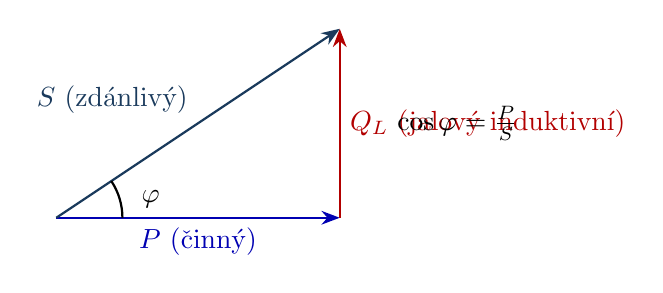
\begin{tikzpicture}[>=Stealth, thick, scale=1.2]
  % Trojúhelník
  \draw[->, blue!70!black] (0,0) -- (3,0) node[midway, below] {$P$ (činný)};
  \draw[->, red!70!black] (3,0) -- (3,2) node[midway, right] {$Q_L$ (jalový induktivní)};
  \draw[->, accent] (0,0) -- (3,2) node[midway, above left] {$S$ (zdánlivý)};
  
  % Úhel
  \draw (0.7,0) arc (0:33.7:0.7);
  \node at (1,0.2) {$\varphi$};
  
  % Popisky
  \node[right] at (3.5,1) {$\cos \varphi = \frac{P}{S}$};
\end{tikzpicture}
\end{center}

% ================================================================
\subsection*{5. Kompenzace jalového výkonu}

Většina spotřebičů v průmyslu (motory, transformátory) má \textbf{induktivní} charakter. To způsobuje vznik induktivního jalového výkonu $Q_L$, který zatěžuje přenosovou soustavu proudem, jenž nekoná práci.

\textbf{Princip kompenzace:} K induktivnímu spotřebiči připojíme paralelně \textbf{kondenzátor} s jalovým výkonem $Q_C$. Protože fázor $Q_C$ míří opačným směrem než $Q_L$, výsledný jalový výkon $Q = Q_L - Q_C$ se zmenší, úhel $\varphi$ klesne a účiník $\cos \varphi$ vzroste (ideálně k hodnotě 0,95 -- 1).

\begin{durazbox}
\textbf{Proč kompenzujeme?}
\begin{itemize}
  \item Snížení ztrát v rozvodech (menší proud při stejném činném výkonu).
  \item Lepší využití výkonu transformátorů a generátorů.
  \item Vyhnutí se pokutám od dodavatele energie za nízký účiník.
\end{itemize}
\end{durazbox}

\begin{center}
\begin{circuitikz}[font=\small]
  \draw (0,0) to[sinusoidal voltage source, l=230\,V] (0,3)
    -- (2,3) to[R, l=$R$] (2,1.5) to[L, l=$L$] (2,0) -- (0,0);
  \draw (2,3) -- (4,3) to[C, l=$C_{komp}$] (4,0) -- (2,0);
  \node at (2, -0.5) {\textit{Induktivní zátěž}};
  \node at (4, -0.5) {\textit{Kompenzace}};
\end{circuitikz}
\end{center}

\begin{vzorcebox}
\textbf{Výpočet kompenzační kapacity:}
\[
Q_C = P \cdot (\tan \varphi_1 - \tan \varphi_2)
\qquad
C = \frac{Q_C}{\omega \cdot U^2}
\]
kde $\varphi_1$ je původní úhel a $\varphi_2$ je požadovaný (kompenzovaný) úhel.
\end{vzorcebox}

% ================================================================
\subsection*{6. Shrnutí – přehled vzorců}

\begin{center}
\begin{tabularx}{0.97\linewidth}{@{} l l l @{}}
\toprule
\textbf{Veličina} & \textbf{Vzorec} & \textbf{Jednotka} \\
\midrule
Úhlová frekvence & $\omega = 2\pi f$ & rad/s \\
Efektivní hodnota & $U = U_m / \sqrt{2}$ & V \\
Induktivní reaktance & $X_L = \omega L$ & $\Omega$ \\
Kapacitní reaktance & $X_C = 1 / (\omega C)$ & $\Omega$ \\
Impedance & $Z = \sqrt{R^2 + (X_L - X_C)^2}$ & $\Omega$ \\
Činný výkon & $P = U \cdot I \cdot \cos \varphi$ & W \\
Jalový výkon & $Q = U \cdot I \cdot \sin \varphi$ & VAr \\
Zdánlivý výkon & $S = U \cdot I$ & VA \\
Účiník & $\cos \varphi = P / S$ & -- \\
\bottomrule
\end{tabularx}
\end{center}

\end{vysvetlenibox}

\end{document}